\documentclass[11pt]{report}
\usepackage{geometry}
\usepackage{graphicx}
\usepackage{subfig}
\geometry{a4paper}
\usepackage{a4}

\usepackage[english]{babel}
\addto\captionsenglish{%
\renewcommand{\chaptername}{Tutorial}}

\usepackage[pdfborder={0 0 0}]{hyperref}

\setlength\parskip{\bigskipamount}
\setlength\parindent{0pt}

\title{VCESS Legal Studies: Units 3 and 4}
\author{Anna, Mariah and Chris}

\begin{document}

\maketitle

\setcounter{tocdepth}{1}
\renewcommand\contentsname{Tutorials}
\tableofcontents

\chapter*{Tutorial Questions}

\section*{Tutorial 1}
\begin{enumerate}
	\item Describe \emph{two} principles of the Australian parliamentary system.
	\item Individuals and groups can influence a change in the law. Explain \emph{one} method they might use.
\end{enumerate}

\section*{Tutorial 2}
Outline whether or not you think the High Court should be allowed to interpret the constitution and why.

\section*{Tutorial 3}
`With their ability to shape the law in relation to specific cases, the courts are far more effective law makers than parliament'. Critically discuss. 

\section*{Tutorial 4}
\begin{enumerate}
	\item List two reasons for a court hierarchy.
	\item The Magistrates' Court can deal with indictable offences heard summarily. What does this mean?
	\item What is the nature of disputes which may be resolved through methods of alternative dispute resolution (ADR)? List two examples of such disputes.
	\item Explain three advantages of ADR over judicial determination and vice versa.
\end{enumerate}

\section*{Tutorial 5}
The inquisitorial system of trial is a far better system of trial compared with the adversary system. Critically discuss. 

\section*{Tutorial 6}
`Pre-trial procedures are designed to speed up the resolution of civil disputes.'
Comment on this statement. In your answer describe one civil pre-trial procedure.

\chapter{Parliament and the Citizen}

\section{The Australian Parliamentary System}

\begin{description}
	\item[Representative Government] The government is composed of Members of Parliament (MPs), elected by the people to represent them.
	\item[Responsible Government] A democratically elected government must be accountable to Parliament and the people. If it loses the confidence of Parliament (specifically, the House of Representatives) then it must resign. Furthermore, ministers are responsible for the actions of their respective departments and must be able to answer questions in relation to them. If a minister is unable to carry out their duties with integrity and propriety, then they too are expected to resign.
\end{description}

\subsection{Separation of Powers}
Under the Australian parliamentary system, power is divided between three distinct branches of government. These are:

\begin{description}
	\item[The Executive] which responsible for the administration and running the business of government. 
	\item[The Legislature] which has the power to enact, amend or repeal legislation.
	\item[The Judiciary] which isresponsible for interpreting the law.
\end{description}

The independence of these branches serves to create a system of checks and balances which limits, in theory, the capacity of governments to abuse their power.

Australia has an imperfect separation of powers. Whilst, strictly speaking, the Governor-General holds executive power, this is in practice exercised by the Prime Minister and Cabinet with the endorsement  of the Governor-General being a mere formality. As a result, the executive and legislature are not completely separate.

\subsection{Structure of Parliament}

The Commonwealth Parliament is made up of the:
\begin{description}
	\item[House of Representatives] a lower house consisting of 150 MPs, representing electorates that each contain approximately the same number of people; and
	\item[Senate] an upper house consisting of 76 MPs -- 12 per state and 2 per territory.
\end{description}

The Victorian Parliament is made up of the:
\begin{description}
	\item[Legislative Assembly] a lower house with 88 MPs representing districts; and 
	\item[Legislative Council] an upper house with 40 MPs representing regions. Each region contains 11 districts.
\end{description}

\subsubsection{The Role of the Lower House}
\begin{itemize}
	\item House of government: the party (or coalition of parties) with a majority of seats in this house may form government. If this does not occur, a party can still form government if it can secure confidence and supply agreements with a sufficient number of MPs. This is known as a minority government.
	\item It is said to be the \emph{peoples' house} because it represents the interests of the general population.
	\item Initiates new laws, amends existing laws and repeals outdated laws
\end{itemize}

\subsubsection{The Role of the Upper House}
\begin{itemize}
	\item The upper house was intended to represent the interests of the state (at a federal level) or regions (at a state level). This is reflected in the makeup of the house where each state is represented equally, regardless of their size of population. However it is important to note that in reality upper house members will vote along party, rather than state/regional, lines.	
	\item House of review: checks legislation passed in the lower house, may amend or reject a bill, uses committees to research and review legislation.
	\item It shares many of the law-making functions of the lower house but often with some important caveats. The Senate (federal upper house) may not initiate bills imposing taxation or some kinds of appropriation and may not amend any bill so as to increase any `proposed charge or burden on the people'.
\end{itemize}

\subsubsection{The Role of the Crown}
Represents the Queen through the Governor-General (Federal level) and Governors (State level). Their roles include:
\begin{itemize}
	\item Ensuring that democratic system (Parliament, electoral system and courts) operates effectively;
	\item Acting as head of state;
	\item Giving royal assent to bills passed by both Houses of Parliament. A process necessary for them to become law;
	\item Designating parliamentary session times, bringing sessions of parliament to an end and dissolving the lower house before an election;
	\item Exercising reserve powers, for example, dismissing a government.
\end{itemize}

\section{Changing Laws}

Law is not static and must change to meet the changing needs of society. There are a number of reasons why this is the case, including:

\begin{description}
	\item[Community attitudes and values] Attitudes and values of people will change over time, such as attitudes towards abortion, and so laws need to change to reflect this.
	\item[Technological progress] Another reason why laws need to change is to keep up to date with technology. Technology is changing at a very fast rate, such as cloning and stem cell research, and the law needs to keep up to date with addressing these advances in technology.
	\item[Recognition of issues] Law may need to change as we gain a greater understanding of environmental issues such as global warming or health issues such as the dangers of smoking.
\end{description}

\subsection{The Victorian Law Reform Commission}
The Victorian Law Reform Commission (VLRC) `is an independent, government-funded organisation that develops, monitors and coordinates law reform in Victoria. It performs a number of functions including:

\begin{itemize}
	\item Receiving law reform proposals from the state Attorney-General and suggesting such proposals itself;
	\item Examining and reporting on proposals to the Attorney-General;
	\item Initiating reviews of minor matters of law reform;
	\item Engaging in research and consulting with experts of a given field;
	\item Undertaking educational programs on any areas of law reform relevant to a reference;
	\item Preparing reports on findings with recommendations for change;
	\item Submitting reports to Parliament and parliamentary committees.
\end{itemize}

\subsection{Influencing Change}
Individuals and groups may influence legislative change in any number of ways, some examples include:
\begin{itemize}
	\item Taking part in opinion polls;
	\item Writing letters to Ministers for Parliament (MP) and Ministers;
	\item Organising and signing petitions;
	\item Joining associations/pressure groups and lobbying MPs;
	\item Taking part in strikes and demonstrations 
	\item Voting a particular party out of government.
	\item Using the media by writing letters to the editor of a newspaper etc.
\end{itemize}

\subsection{The Legislative Process}
The process for the passage of a bill through Parliament is as follows:

\begin{description}
	\item[First Reading] The long title is read, the Bill is put on the agenda and copies of the Bill are circulated.
	\item[Second Reading] The relevant minister makes a speech outlining the purpose of the Bill. An explanatory memorandum is presented which explains the reasons for the Bill and outlines its provisions.	
	\item[Consideration in Detail] The bill may be referred to the Committee of the Whole House, or a smaller committee consisting of a few designated members. Each clause of the bill is examined in detail and amendments may be proposed.
	\item[Third Reading] Debate at this stage is rare and usually restricted to matters contained in the clauses and schedules of the bill. When the motion has been agreed to, the Clark reads out the long title of the bill, this signifies that the bill has passed the house.
	\item[Certification] The Bill is certified by the Clerk of Parliaments after it has passed through both houses.
	\item[Royal Assent] The Bill is presented to the Governor-General for her signature.
	\item[Proclamation] The law comes into effect on the day stated in the Act, on a day proclaimed by the Governor-General or, if neither occurs, 28 days after royal assent.
\end{description}

Note that the above steps must be repeated for the other house (the one in which the bill did not originate). If any amendments are made then this must be communicated to the originating house so that the bill can be passed in its new form. To become law, both houses must pass the bill in the same form.

\subsection{Strengths and Weaknesses of Parliament as a Law-Making Body}
\subsubsection{Strengths}
\begin{itemize}
	\item Parliament can investigate a whole topic and make a wide ranging set of laws;
	\item It has access to specialist information and is therefore able to keep up with changes in society;
	\item Provides a public arena for debate and argument;
	\item Able to involve the public in law-making;
	\item Can change the law as the need arises;
	\item Democratically elected and therefore accountable to the people;
	\item May delegate its law making power to a bodies such as statutory authorities and local councils;
	\item It can act quickly to introduce new legislation when necessary.
\end{itemize}

\subsubsection{Weaknesses}
\begin{itemize}
	\item The investigation and implementation of a new law, and the passing of legislation is time consuming;
	\item Parliament is not always able to keep up with changes in society;
	\item There may be too many delegated bodies making law in the same area which may lead to fragmentation or lack of scrutiny and consultation;
	\item It is not always possible to change the law in accordance to changing values in society;
	\item Political considerations rather than the merits of a bill might effect the way MPs vote;
	\item Parliament is not always sitting so changes in the law may have to wait some time;
	\item Changes in the law may involve financial outlay, which may not be economically viable at the time;
	\item Parliament has the capacity to pass retroactive laws. Criminalising past actions which may otherwise have been perfectly legal.
	\item The upper house has the capacity to obstruct legislation;
	\item Cabinet's legislative proposals may dominate law making by Parliament particularly when the government controls both houses.
\end{itemize}

\chapter{The Constitution and Rights}

\section{Division of Power}

The Commonwealth constitution divides law-making powers between the Commonwealth and the states. 

\subsection{Specific Powers}
Under the Constitution, Parliament holds certain powers to `make laws for the peace, order and good government of the Commonwealth.' These powers can belong to one of a number of categories.

\begin{description}
	\item[Exclusive powers] are law-making powers that can only be exercised by the Commonwealth Parliament and no other body. These are specific powers listed in the Constitution that are made exclusive to the Commonwealth. For example:
	\begin{itemize}
		\item Defence, under s 51(vi) and made exclusive by s 114.
		\item Currency, under s 51(xii) and made exclusive by s 115.
	\end{itemize}
	\item[Concurrent powers] are held by both the Commonwealth and state parliaments. For example:
	\begin{itemize}
		\item Marriage, under s 51(xxi)
		\item Taxation, under s 51(ii). Note that, whilst the general power to tax is concurrent, under s 90 `duties of customs and of excise' are made exclusive to the Commonwealth.
	\end{itemize}
	\item[Inconsistencies]  If there is an inconsistency or conflict between state and Commonwealth laws in a concurrent area of power, s 109 states that the state law `shall, to the extent of the inconsistency, be invalid.'
\end{description}

\subsection{Residual Powers}
Residual powers are those not mentioned in the Constitution at all. As a result, the Commonwealth has no power to legislate in these areas. Section 107 ensures that the states retain the power to legislate with respect to residual matters. These law-making powers cover areas such as public transport, education and health.

\subsection{Referral of Power}
The states may elect to refer a residual power to the Commonwealth in which case Parliament will be able to legislate in respect to residual matters under s 51(xxxvii).

This was the case with law making regarding ex-nuptial (outside marriage) children in family law matters. The Commonwealth has the power to legislate in maters of family law including the custody of children in divorce but not in relation to the children of unmarried parents. The states subsequently referred the power to make laws in this area to the Commonwealth.

\section{Restrictions on Law-Making Powers}
The Constitution imposes a number of restrictions on the law-making powers of the Commonwealth and state parliaments.
\begin{itemize}
	\item Section 51(xxxi) states that the acquisition of property by the Commonwealth must be on �just terms�. Note that this restriction does not apply to the states although many state constitutions contain similar protections.
	\item Section 80 requires that trials for an offence under any Commonwealth law must be by jury.
	\item Section 92 guarantees free trade between the states.
	\item Section 99 prevents the Commonwealth giving preference to any one state.
	\item Section 116 prevents laws establishing a religion, requiring religious observance, imposing a religious test or prohibiting the free exercise of religion.
\end{itemize}

\section{Changing the Constitution}
The wording of the Constitution may only be changed through a referendum as set out in s 128. The process for changing the wording of the Constitution is as follows:
\begin{enumerate}
	\item A bill setting out the proposed change is introduced into either house of Parliament. It must pass through both Houses of Parliament before the referendum can be put to the people.
	\begin{enumerate}
		\item If the bill is rejected by one house more than once, s 128 gives the Governor-General the discretion to submit the referendum to the people anyway.
	\end{enumerate}
	\item The people of the states and territories vote YES or NO to the proposal. In order for the referendum to pass, it must receive a double majority. That is to say, it must be supported by a majority of the states and by a majority of the people.
	\begin{enumerate}
		\item If the proposal concerns on state in particular, it is necessary for the referendum to win the support of that state.
	\end{enumerate}
	\item If the referendum passes, it is presented to the Governor-General for royal assent, after which the change is made.
\end{enumerate}

\subsection{The Success of Referenda}
Referenda are difficult to pass. Since federation, there have been 44 proposals of which only eight have been successful. There are a number of factors that contribute to this difficulty, including:
\begin{itemize}
	\item The requirement of a double as opposed to a simple majority.
	\item Lack of bipartisan support for most proposals.
	\item Suspicion, confusion or indifference to the proposal amongst voters. 
	\item Voters and state governments may not wish to increase the power of the Commonwealth at the expense of the states, the focus of many such proposals.
\end{itemize}

\subsubsection{Examples of Successful Referenda}
\begin{description}
	\item[The 1946 referendum on social services] gave the Commonwealth Parliament power to legislate on a wide range of social services (s 51(xxiiiA)), an area that had previously been a residual power.
	\item[The 1967 referendum on the Aboriginal people] removed the words `other than Aboriginals' from s 51(xxvi) and removed the restriction on counting Aboriginal people in national or state censuses. This increased the law making power of the Commonwealth on issues relating to Aboriginal people.
\end{description}

\section{The High Court}

The High Court was established under Section 71. Under Section 76, it has the power to hear disputes arising from the Constitution and those involving its interpretation. The Court does not change the Constitution directly, but adds meaning to it through its decisions and thus affects the balance between federal and state power. Constitutional conflict may arise when:
\begin{itemize}
	\item An individual challenges the power of federal parliament to legislate on matters that effect them;
	\item The federal or state parliaments are in dispute over law making powers. One side may claim the other has passed a law that goes beyond its constitutional power.  
\end{itemize}

The High Court deals with constitutional disputes arising over concurrent areas of power. It determines if the states and Commonwealth are acting within their powers. Some reasons for disputes are:
\begin{itemize}
	\item Wording may be vague, complex or unclear;
	\item Wording may have more than one meaning or change over time;
	\item The meaning of a word may differ according to circumstance;
	\item The statute may not cover all possible future applications.
\end{itemize}

\subsection{The First Uniform Tax Case (1942)}
During the Second World War, the Commonwealth decided that it needed additional revenue to help fund the war effort. To this end, legislation was passed to prevent the states from levying income tax and to make itself the sole income tax collector. Although comprising a number of different acts, the end result was that:

\begin{itemize}
	\item Commonwealth income tax levels were increased to match what the federal and state governments combined had charged.
	\item A grant would be provided to each state equal of an amount equal to what it would have raised through its own income tax on the condition that it did not levy such a tax.
	\item Taxpayers were required to pay the Commonwealth income tax before any state income tax.
	\item The states were required to transfer all staff, offices, furniture and records used to collect income tax to the Commonwealth.
\end{itemize}

South Australia, Victoria, Queensland and Western Australia challenged the laws. The High Court ruled in favour of the federal government. Whilst the legislation raised tax rates to a level that made it politically impossible for the states to impose their own, this did not constitute direct coercion. States still had a choice as to whether they would accept the Commonwealth grants.

This decision has had a profound effect on the Commonwealth-state relations. The consequence is that the states have become increasingly dependent on federal grants in order to function and, by attaching conditions to this money, the federal government has been able to have an even greater influence in residual matters.

\subsection{The Tasmanian Dam Case (1983)}
The Tasmanian government intended to build a dam near a junction of the Franklin River for the purposes of generating hydroelectricity. In response, the federal government passed the \emph{World Heritage Properties Conservation Act} in an attempt to prevent its construction. The governments of Tasmania, Victoria, New South Wales and Queensland challenged the federal law in the High Court.

Since both the environment and the supply of electricity are areas of residual power, the Commonwealth claimed that the law was passed pursuant to the external affairs power (s 51(xxix)). Specifically, for the purposes of giving effect to Australia's obligations under the \emph{Convention Concerning the Protection of the World Cultural and Natural Heritage}. The Franklin River had been declared a world heritage site in 1982. The High Court found that the federal law was valid and that Parliament could pass legislation in support of international agreements to which Australia is a party. 

This case is an interesting example of the High Court's ability to impact on the division of powers because of its potential to allow the Commonwealth to intervene in any area of residual power affected by an international treaty to which Australia is a signatory, including human rights.

\section{Rights Protection}
The Constitution provides for the protection of rights in a number of ways.
\begin{description}
	\item[Structural Protections] are mechanisms or systems that indirectly protect human rights by preventing abuse of power. These include the separation of powers and representative government and reflect that there are checks and balances built into the constitution that prevent human right abuses. 
	\item[Express Rights] are specifically stated in the constitution and include:
	\begin{itemize}
		\item Freedom of religion (s 116);
		\item Freedom of interstate trade and commerce (s 92);
		\item Provisions against the discrimination against people based on their state of residence (s 117);
		\item Property can only be acquired on `just terms' (s 51(xxxi));
		\item Trial by jury for Commonwealth indictable offences (s 80). Note that this is very limited because most indictable offences are crimes under state law. Furthermore, the Commonwealth can subvert this protection by legislating for an offence to be summary rather than indictable.
	\end{itemize}
	\item[Implied Rights] are not expressly stated in the Constitution but rather, implied through its wording. These include rights such as freedom of political communication (see \emph{Lange v Australian Broadcasting Corporation}). 
\end{description}

\subsection{Lange v Australian Broadcasting Corporation}
David Lange, the Prime Minister of New Zealand, was the subject of a report on the ABC program, Four Corners. He later brought defamation proceedings in respect of the broadcast.

The High Court in \emph{Australian Capital Television v The Commonwealth} had earlier recognised the existence of a right to free political communication. In affirming its earlier finding, the High Court also sought to clarify the nature of the right. It found freedom of political communication to be an `indispensable incident' of the system of representative government established by the Constitution. This freedom ensured the `capacity of, or the opportunity for, the Australian people to form the political judgement required for their constitutional functions' outlined in ss 7, 24, 64 and 128 of the Constitution.

It should be noted that, whilst a broad interpretation was taken as to what constitutes `political communication', the court did not find an implication of a general right to free speech.

\subsection{Rights Protection in South Africa}
\begin{itemize}
	\item The South African legal system contains a far greater level explicit rights protection than that of Australia. The South African Bill of Rights was introduced 1996, there is no \emph{constitutionally protected} Bill of Rights in Australia.
	\item This document serves to \emph{entrench} the rights, this means that a right can only be abolished if the Constitution is amended (note that the five express rights mentioned above are entrenched in the Australian constitution).
	\item The rights are fully enforceable. This means that legislation which infringes any of those rights can be declared invalid by the Constitutional Court. Similarly, Australia�s constitutionally protected rights are fully enforceable 
-- any legislation which infringes one of the rights can be declared invalid by the High Court. 
	\item It contains a comprehensive list of rights whereas Australia�s Constitution contains just the five express rights and several implied rights (see \emph{Lange}).
	\item A special feature of the South African Bill of Rights is its inclusion of economic, social and cultural rights. Australia�s protected rights do not include these sorts of rights, although it might be argued that s 92 amounts to the protection of an economic right.
	\item Courts are required to interpret statutes in accordance with the Bill of Rights. While Australia has had examples where High Court judges have referred to international human rights standards when developing the common law (for example, in \emph{Mabo}), this has not been an approach generally adopted by the court, 
particularly the current court. 
	\item Rights can be limited where justified in free and democratic society. In Australia, there is no Bill of Rights containing such a provision.  
	\item In Australia a person requires \emph{standing} to take bring an action for a breach of a right. Essentially this means that the matter must relate to them or their interests. In South Africa actions may be brought in the public interest.
\end{itemize}

\chapter{Role of the Courts in Law-Making}

\section{The Doctrine of Precedent}

The doctrine of precedent is a common law (i.e. judge made law/case law) principle which governs the ability of judges to make new law. Before you can understand how the doctrine of precedent works, you must know something about the court hierarchy:
\begin{figure}[htbp]
  \centering
  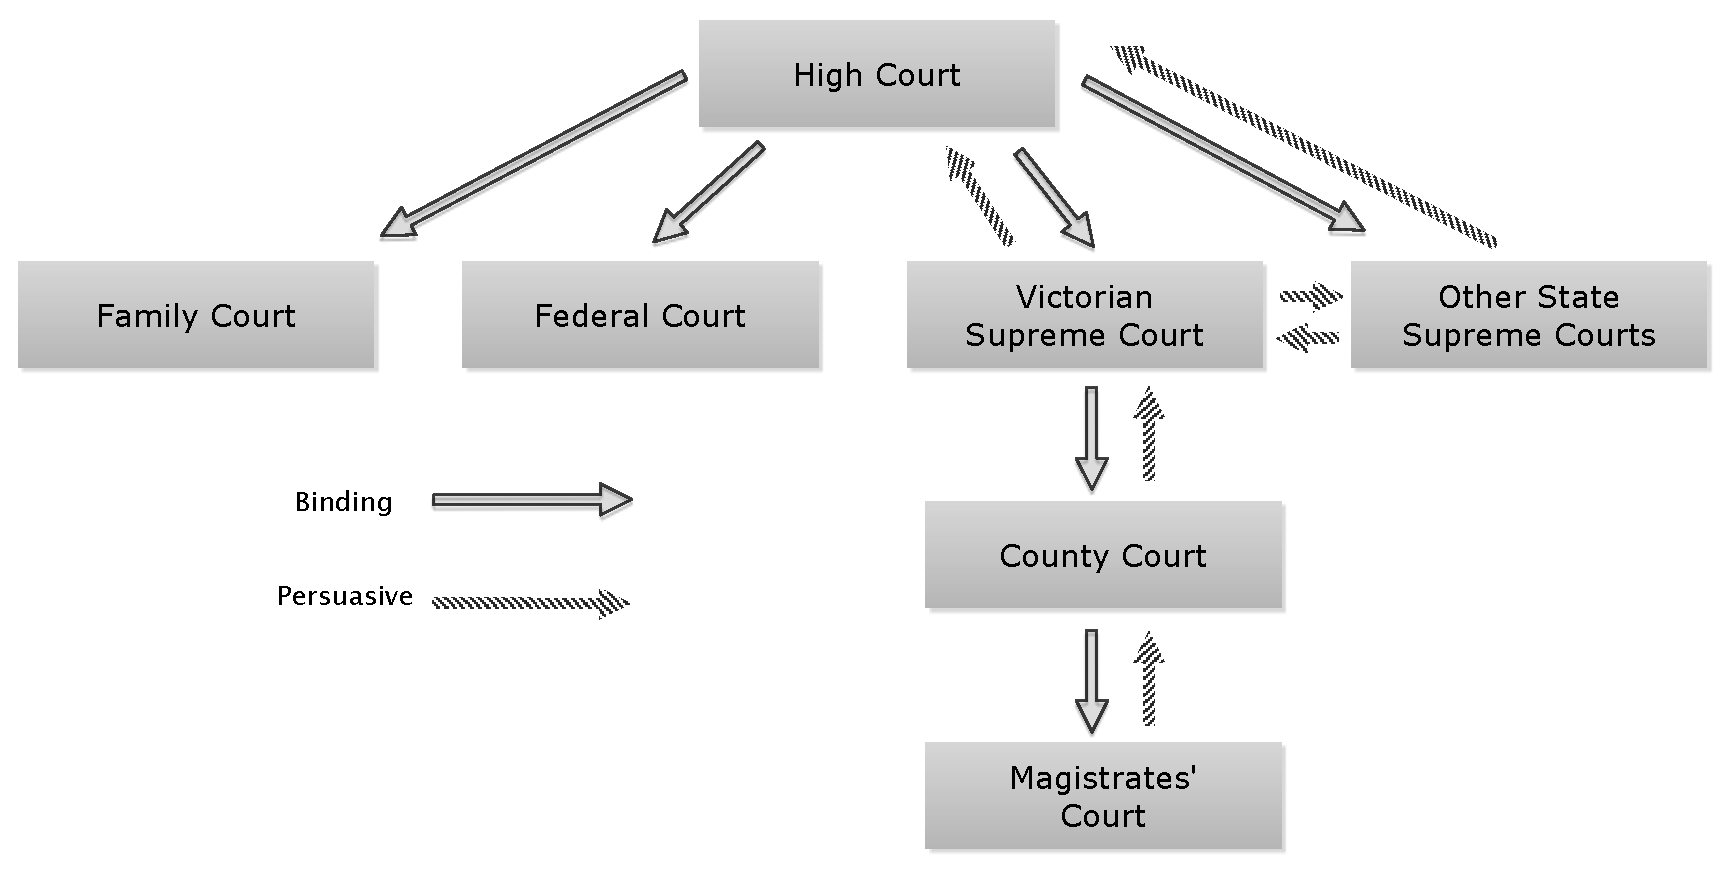
\includegraphics[scale=0.5]{precedent_diagram.pdf}
  \caption{This diagram shows the effect that a decision from a higher court has on a lower court. Decisions from higher courts are binding on lower courts, while decisions from lower courts are, at most, persuasive on higher courts. }
\end{figure}

\subsection{Key Features}
Key features of the doctrine include:
\begin{itemize}
	\item It is developed through court decisions and occurs in the course dispute of resolution.
	\item It operates according to the principle of \emph{stare decisis}, where decisions or precedents set in higher courts are binding on similar cases in lower courts in the same hierarchy.
	\item \emph{Ratio decidendi} is the part of the judgement that is binding on similar cases in lower courts.
	\item A higher court is able to \emph{overrule} a decision made in a lower court.
	\item A decision of a higher court remains law until it is overruled by a higher court  or altered by an Act of Parliament.
	\item The High Court may overrule its past decisions.
	\item A decision may be \emph{reversed} on appeal in which case it is no longer binding. 
	\item A judge may avoid following a precedent if the material facts of the case before them can be \emph{distinguished} from those of the previous case.
	\item A single judge is not bound by the decisions of a single judge of the same court.
	\item \emph{Obiter dictum} is a statement made in passing by the judge. Such a statement is not directly relevant to the point of law in question or the binding part of a precedent (the \emph{stare decisis}). However, such statements may act as persuasive precedents in future cases.  
	\item Decisions in lower courts may act as persuasive precedents on decisions in courts higher in the same hierarchy.
	\item By \emph{disapproving} an earlier decision, a higher court can indicate to lower courts in the same hierarchy that a decision should no longer be regarded as a good law.
\end{itemize}

\section{Statutory Interpretation}
Statutory interpretation is a process whereby judges determine the application of an act to a particular case and how the law applies to a specific set of circumstances. Judges interpret acts of parliament to give the words meaning. Statutory interpretation may only occur when a case involving a dispute about the meaning or application of act appears before a court. The given definition or interpretation of a particular word is valid only for the statute interpreted.

\subsection{Reasons for Statutory Interpretation}
\begin{itemize}
	\item The wording of statutes may be complex or unclear;
	\item The meaning of words may differ in different circumstances or over time;
	\item The purpose of the statute may not be sufficiently clear or may not cover all future applications;
	\item Subsequent parliamentary amendments to the Act may have distorted the original meaning/purpose of the Act.
\end{itemize}

\subsection{Effect of Statutory Interpretation}
Statutory interpretation does not change the actual wording of an act. However, the way an act is interpreted may have the following effects:
\begin{itemize}
	\item It can set a precedent that will be either binding or persuasive on other judges depending on the position of the interpreting court in the hierarchy. In this way statutory interpretation is another way judges make law. 
	\item A wide interpretation may extend the law or conversely a narrow interpretation may restrict the law 
\end{itemize}

\section{Strengths and Weaknesses of Law-Making through the Courts}

\subsection{Strengths}
	\begin{description}
		\item[A decision must be made] A court must reach a decision, so it can change law quickly or can fill a gap in the law if a relevant case is brought before it.
		\item[Flexibility] Courts can keep the law from becoming too inflexible by distinguishing, overruling and reversing previous decisions and giving meaning to words in statutes.
		\item[Independent of political process] Judicial decisions are not influenced by outside pressures due to the independence of the judiciary established through the separation of powers.
		\item[Courts, in applying the law, determine its day-to-day operation] Courts may interpret the words of an act of parliament to provide a more just result to the case at hand .
		\item[Predictability] The doctrine of precedent limits the possibility of prejudices or bias influencing judicial decisions.
		\item[Access to change] The appeals procedure allows for a review of new decisions.
	\end{description}

\subsection{Weaknesses}
	\begin{description}
		\item[Inflexibility] A court can not change a law unless a case is brought before it.
		\item[Rigidity] Courts may be bound to an outdated precedent which may lead to unjust results or some judges may be conservative and reluctant to change laws.
		\item[Cost] Bringing legal action can be very expensive for parties involved.
		\item[Parliamentary Supremacy] Parliament can override the common law.
		\item[Undemocratic] Judges are not elected, which means that this is not a democratic system of law-making.
		\item[Law-making not the main role of the court] Law making is a secondary role of the courts -- their primary role is to settle disputes and decide if laws have been broken.
	\end{description}

\section{Relationship between Courts and Parliament in Law-Making}
Parliament is the supreme law-making authority. The courts receive their powers through acts of Parliament.

\begin{itemize}
	\item Courts tend to fill the gaps left by statutes;
	\item Courts are needed to make law or clarify issues on matters that arise on an ongoing basis;
	\item Judicial interpretation of legislation may establish a precedent whilst parliament can legislate to overrule that precedent
	\item Laws may need to be challenged or interpreted -- courts do this;
	\item Courts are important in developing law in areas where Parliament has lacked the will or capacity to do so;
	\item Many areas of law are still predominantly common law. Some consist of a combination of common law and statute law;
	\item Law making is the central role of Parliament; it is secondary for the courts;
	\item Statute law has become a significant source of law, particularly in complex and developing areas of law.
\end{itemize}

\chapter{Methods of Dispute Resolution}

\section{The Court Hierarchy}
The court hierarchy exists to:
\begin{itemize}
	\item Provide a court at each level with particular expertise, skill and proficiency 
	\item Allow a system of appeals to operate 
	\item Facilitate the operation of the doctrine of precedent 
	\item Provide administrative convenience and more efficient use of resources 
\end{itemize}

\subsection{The Victorian Court Hierarchy}

\subsubsection{The Magistrates' Court}

\begin{itemize}
	\item Original Jurisdiction (Criminal): summary offences (minor offences), indictable offences heard summarily (heard without a jury). Also holds committal hearings.
	\item Original Jurisdiction (Civil): cases where amount is up to \$100,000. When less than \$10,000 the case is referred to arbitration.
	\item This court has no appellate jurisdiction.
\end{itemize}

\subsubsection{County Court}

\begin{itemize}
	\item Original Jurisdiction (Criminal): almost all indictable offences except those of a very serious nature, such as murder.
	\item Original Jurisdiction (Civil): Unlimited damages amount for all civil matters.
	\item The court can hear appeals from the Magistrates' Court on criminal matters. It generally cannot hear appeals on civil matters.
\end{itemize}

\subsubsection{Supreme Court}

\begin{itemize}
	\item Original Jurisdiction
	\begin{itemize}
		\item Criminal: very serious criminal offences such as murder and treason.
		\item Civil: unlimited -- cases about large disputes over personal injury, money and business disagreements. Generally hears claims over \$200,000.
	\end{itemize}
	\item Appellate Jurisdiction
	\begin{itemize}
		\item Trial Division: Appeals on points of law from the Magistrates' Court. These are heard by a single judge of the Supreme Court.  
		\item Court of Appeal
		\begin{itemize}
			\item Criminal: from a single judge of the County Court and Trial division of the Supreme Court. 
			\item Civil: from a single judge of the County Court and Trial division of the Supreme Court and from the Victorian Civil and Administrative Tribunal (VCAT)
		\end{itemize}
	\end{itemize}
\end{itemize}

\section{Methods of Dispute Resolution}
\emph{Judicial determination} is a dispute resolution process whereby parties to a legal dispute present evidence and submit arguments to a judge, magistrate, or VCAT member, who then makes a legally binding decision.

\subsection{Alternative Dispute Resolution Methods}
Alternative Dispute Resolution methods, as the name suggests, provide an alternative to dispute resolution through judicial determination. These methods are often called `primary dispute resolution', suggesting that some civil disputes ought to be settled in this way initially.

\begin{description}
	\item[Abandonment] Party decides not to pursue a matter.
	\item[Conciliation] Parties come before an arbitrator who controls the process of dispute resolution and makes a binding decision. The arbitrator is an independent third party who, unlike a judge, is not bound by the rules of evidence and procedure.
	\item[Mediation] The parties come before a conciliator, an independent 3rd party who usually possesses expert knowledge and attempts to help parties settle the dispute. The conciliator listens to both sides of the dispute and makes suggestions on how to solve the dispute but does not make the final decision.  Decisions are based on parties reaching a mutual agreement. Conciliation is compulsory prior to some court proceedings such as civil matters in the Magistrates' Court.
	\item[Negotiation] Parties engage in dialogue with one another in an attempt to find a mutually satisfactory decision. Legal representation or a 3rd party are not usually used and decisions are not legally binding.
	\item[Self-help] A party decides to find a solution themselves, without seeking outside help -- e.g. they cut off their neighbour�s overhanging tree branches. 
\end{description}

\subsubsection{Strengths of ADR}
\begin{itemize}
	\item Confidential and flexible -- potential to offer more creative solutions to civil disputes;
	\item Less formal (rules of evidence and procedure do not apply) and much cheaper when compared to formal litigation;
	\item Less time consuming than formal litigation;
	\item May aid to preserve relationships between parties whose circumstances require the maintenance of an ongoing relationship e.g. neighbours;
	\item Most methods of ADR provide an opportunity for parties to find their own solution to the problem rather than having a solution imposed on them.
\end{itemize}

\subsubsection{Weaknesses of ADR}
\begin{itemize}
	\item Not suitable unless all parties are willing to participate;
	\item Not suitable for all parties -- particularly those who are determined to have `their day in court';
	\item Not suitable if one party feels intimidated by the other;
	\item Dispute may end up in court resulting in increase in overall cost and time spent resolving the it.           
\end{itemize}

\section{Tribunals}
Reasons for tribunals
\begin{itemize}
	\item Usually cheaper than courts and decisions are usually quicker;
	\item Generally seen as less threatening and more accessible than courts;
	\item Jurisdiction of tribunals is generally more specialised than courts;
	\item The ability to appeal against a decision of a tribunal is limited (VCAT appeals go all the way to the Supreme Court).
\end{itemize}

\subsection{Victorian Civil and Administrative Tribunal (VCAT)}
The role of VCAT is aiming to facilitate:
\begin{enumerate}
	\item Timely decisions;
	\item Low cost proceedings;
	\item Expert determination;
	\item Accessible processes; and
	\item Independent operation.
\end{enumerate}

\subsubsection{Structure}
VCAT consists of three divisions. An Administrative Division, Civil Division and Human Rights Division.

Each division has a number of lists. Three examples are:
\begin{description}
	\item[Anti-discrimination list] located in the human rights division. Determines complaints from people who feel they have been discriminated against in particular areas (eg. employment, education, provision of goods and services, accommodation, membership of a club) and on particular grounds (eg. Age, marital status, impairment, industrial activity, lawful sexual activity, pregnancy, physical features, religion etc.).
	\item[Residential Tenancies list] located in the Civil division. Was set up to hear disputes between landlords and tenants covering leases, bonds, rents, damage, repairs to property and eviction. Can hear disputes of up to \$10,000 on residential properties.
	\item[Civil claims list] also located in the Civil division. Deals with smaller claims. Resolves disputes between consumers and traders relating to the provision of goods and services. Can hear complaints regarding claims up to the value of \$10,000.
\end{description}

VCAT decisions are binding and enforceable through the courts. Stages in dispute resolution through VCAT may include mediation, compulsory conferences and hearings. 

\section{Comparison of the Courts, Tribunals and ADR}
Some key issues when comparing the operation of courts, tribunals and ADR are:
\begin{itemize}
	\item ADR, except arbitration is voluntary compared to formal court hearings;
	\item Tribunals and ADR are usually more cost effective than court hearings;
	\item Mediators assist parties to discuss all issues, explore possible solutions and reach a decision;
	\item Whereas mediation in encouraged by the courts, it is not undertaken by the judge or magistrate. In a court hearing, a judge or magistrate (and jury where applicable) hears evidence put forward by each party and then makes a decision that is binding on both parties;
	\item Strict rules of evidence and procedure, found in court proceedings, do not apply to tribunals or ADR;
	\item If parties reach a settlement in ADR, an agreement can be drawn up incorporating the terms of the settlement. Court decisions on the other hand, are imposed;
	\item Tribunals and ADR are available only for civil matters and ought not to be used in situations where parties cannot engage in negotiation or mutual agreement. Court hearings are required in criminal cases;
	\item All major courts encourage mediation and in some cases order it. 
\end{itemize}

\chapter{Court Processes and Procedures I}

A number of criteria are required for an effective legal system to exist:
\begin{itemize}
	\item Entitlement to a fair and unbiased hearing;
	\item Effective access to mechanisms for the resolution of disputes;
	\item Timely resolution of disputes without excessive delays;
	\item Recognition of prevailing values and human rights.
\end{itemize}

\section{The Adversary System}
In criminal cases, the courts use an adversary system of trial. The major features are:
\begin{description}
	\item[Role of parties/party control] each party -- the prosecution and defence -- is responsible for the preparation and presentation of their own case. They may present witnesses and evidence to support their case and present it in the best possible light. They are also allowed to question witnesses and evidence presented against them.
	\item[Professional representation] both parties have the right to legal representation. People who cannot afford legal representation are entitled to receive legal aid. There is an assumption that both parties are equally able to represent their cases however legal representation varies and in many cases parties who are financially better off are able to hire more skilled and/or experienced legal representatives. This may alter the outcome of the case. 
	\item[Role of the judge] the judge or magistrate's role is as an impartial adjudicator who does not argue for or favour any particular side. Their role is to ensure that all parties abide by the rules of evidence and procedure. The judge is also responsible directing the jury on a point of law and sentencing the defendant in the event that the jury finds them to be guilty. Where there is no jury, the judge is required to decide the guilt of the offender. 
\end{description}

\section{Rules of Evidence and Procedure}
\begin{description}
	\item[Rules of Procedure] govern the conduct of the trial and ensure that each party has an equal opportunity to present their case. Both parties may call witnesses to give their testimonies in court. This involves examination in chief where a witness gives evidence for the first time by answering questions. The other side may then question a witness -- this is called cross-examination. This may reveal weaknesses in the witness�s testimony.  However the initial party who brought forward the witness then has the opportunity to bolster their case by asking further questions to the witness through re-examination of the witness.
	\item[Rules of Evidence] govern the type and standard of evidence that parties may present in court. Most evidence presented is in the form of oral witness testimony but may also include pieces of physical evidence. Any evidence presented must be legally collected. The rules of evidence restrict parties in presenting some types of information. Pieces of information usually excluded from admissible evidence include:
	\begin{itemize}
		\item Evidence collected illegally: e.g. when police obtain evidence without a warrant;
		\item Hearsay evidence: when a witness repeats, as part of their testimony, what they heard from a third party, rather than what they saw or heard themselves. This is inadmissible;
		\item Opinion evidence is when a witness uses their opinion as evidence. This is generally not allowed, unless the witness is considered an expert in their field e.g. a psychiatrist giving their opinion on the mental state of the accused. It may also be used in the case of a parent testifying that the behaviour of their child was out of character;
		\item Prior convictions: records of past offences that the accused has been found guilty of (or convicted for). Generally this can not used as evidence, but in some cases it may be used to establish that a person has a tendency to behave in a certain way -- this is called propensity evidence;
		\item Privileged information: private information which can generally not be given as evidence without consent e.g. conversations between lawyers and their clients cannot be given in court without the clients permission;
	\end{itemize}
	\item[Burden of proof] the responsibility is placed on the party bringing the case to court to prove the case against the other party. In criminal cases the burden lies with the prosecution who must prove that the accused is guilty. This links with the principle of innocent until proven guilty. 
	\item[Standard of proof] the extent to which the party bringing the case to court must prove the case.  In criminal trials the standard of proof is beyond reasonable doubt. This means that a jury must either come up with a unanimous verdict or an absolute majority verdict.
\end{description}

\subsection{Strengths and Weaknesses of the Adversary System}

\subsubsection{Strengths}
\begin{itemize}
	\item Individuals are responsible for the conduct of their own affairs. This means that they can be sure that they have done everything in their power to succeed in winning the case;
	\item Rules of evidence and procedure set down for both parties ensure that both are on a even playing field; 
	\item The system has stood the test of time and the community is generally understood to have confidence in the system;
	\item Those affected directly bear the costs;
	\item All important evidence is put forward because both parties are responsible for putting forward the best possible case for themselves;
	\item The judge is an impartial and independent umpire;
	\item The standard and burden of proof protect the innocent -- ensures that the accused is innocent until proven guilty; may only be convicted if evidence is sufficient.
\end{itemize}

\subsubsection{Weaknesses}
\begin{itemize}
	\item Important facts may be left out because each side may only present favourable evidence;
	\item Cost of resolving criminal matters through the courts is high for all the parties involved. This includes the cost of legal representation;
	\item Appearing in court unrepresented may be detrimental and legal aid is provided. However legal aid may not be enough and it is not accessible to all who may need it;
	\item The legal skill and experiences of magistrates and judges may be under-utilised;
	\item Courts operate in very formal environments � this may be intimidating to some witnesses whose oral evidence is often relied upon to prove the guilt or innocence of the accused. 
\end{itemize}

\section{The Inquisitorial System}
This system is used in countries such as Germany, Greece, France and Indonesia. Notable features include:
\begin{itemize}
	\item Active involvement by the judge in the case and trial. A judge may question witnesses and determine which witnesses and evidence are admissible;
	\item The rules governing procedures (called codes) are set down by legislation and court made law plays no part in determining procedures;
	\item Greater reliance on documentary evidence. Witnesses have more freedom to describe events in their own words;
	\item The court is not restricted solely to the issues and evidence placed before it by the parties when making a decision; 
	\item Legal representation may not be essential in all cases.
\end{itemize}

\section{Possible Reforms to the Adversary System}
Could implementing part of the Inquisitorial system improve our adversary system?
\begin{itemize}
	\item Greater investigative role of the judge may lead to a greater emphasis on ascertaining the truth;
	\item Greater use of written statements may reduce costs and delays;
	\item Less formal conduct of the trial and absence of strict rules of evidence and procedure means that witnesses may give evidence in narrative form. This could be prevent useful evidence from being excluded since the witness tells all relevant parts of the story. Counsel can still question witnesses;
	\item Legal representation may not be essential diminishing the issue of legal costs and disadvantage as a result of lack of representation.
\end{itemize}

Other possible reforms include:
\begin{itemize}
	\item Simplification of the rules of evidence and procedure;
	\item Encouragement of alternative methods of dispute resolution;
	\item Greater availability of legal aid;
	\item Increased spending on the legal system as a whole.
\end{itemize}

\section{The Jury System}
The jury system is based on the ideas that all individuals in the community are responsible for the administration of justice. This means that every person has the right to be tried in accordance with the values held generally by the community. Therefore the aim of the process used to choose jurors is to provide a cross-section of the community.

Any person whose name is on the electoral role can be called for jury duty. However there are exceptions. 

In criminal cases in the Supreme and County Courts, a jury of 12 will be used. Both parties may challenge potential members of the jury during the empanelment process (peremptory challenges and/or for cause challenges are available to both parties). The role of the jury is to hear all the evidence presented and decide whether the accused is guilty or not guilty beyond reasonable doubt. This is called the verdict. It is the judge's role to impose sanctions.  If a unanimous verdict -- 12 out of 12 jurors agree on the verdict -- has not been reached after 6 hours of jury deliberation, the judge may agree to a majority verdict -- where 11 out of 12 jurors agree on the verdict. 

\subsection{Strengths and Weaknesses of the Jury System}

\subsubsection{Strengths}
\begin{itemize}
	\item Jury decisions reflect the views of the community;
	\item Juries are meant to be independent or impartial;
	\item Ensure the law remains in touch with ordinary people;
	\item Free from political interference;
	\item Has stood the test of time -- people have confidence in the system.
\end{itemize}

\subsubsection{Weaknesses}
\begin{itemize}
	\item Reasons do not have to be given when a jury comes up with a verdict;
	\item People can be excused or challenged -- this means that juries are never a true cross section of the community;
	\item Jurors may fail to understand or recall important evidence, which may be complex or technical.
\end{itemize}

\section{Difficulties in using the Legal System}
\begin{itemize}
	\item Delays in legal processes and procedures -- excessive delays between arrest and trial cause stress and fail to provide speedy justice;
	\item Existence of appropriate structures for the resolution of cases -- even though a range of structures are in place, problems still exist concerning inadequate facilities and enough facilities for all people needing access to legal structures e.g. in rural areas;
	\item Trial, pre-trial and post trial civil and criminal procedures -- see above;
	\item Cost of legal representation;
	\item Provision of Legal Aid -- only available to the very needy. Merit tests and funding are also an issue.
\end{itemize}

\section{Recent Changes and Recommendations}
\begin{itemize}
	\item Increased spending on the courts;
	\item Increased number of judges and greater diversity of judicial appointment;
	\item Changed jurisdictions to the courts e.g. Increased civil jurisdiction of the Magistrates' Court;
	\item Established specialised divisions of the Magistrates' court to deal with specific issues e.g. Koori Court and Family Violence Court;
	\item Increased and continued use of ADR mechanisms;
	\item Reducing delays in the time cases come to court;
	\item Increased consideration of social and cultural differences.
\end{itemize}

\chapter{Court Processes and Procedures II}

\section{Criminal Pre-trial Procedures}
\begin{description}
	\item[Police powers and the rights of individuals] \hfill
	\begin{itemize} 
		\item Police collection of evidence which may include searching a premises upon the issue of a warrant;
		\item Police questioning which may involve detaining the accused for a reasonable time to take record of an interview;
		\item Filing a charge, arrest or summons;
		\item Arrest -- with or without a warrant;
		\item Police are entitled to take fingerprints, blood and body samples;
		\item Accused has the right to contact another person (friend, relative, lawyer);
		\item Suspects generally have a right to silence and cannot be forced to take part in a police line up;
		\item Individuals have a right to an interpreter if their English is deficient.
	\end{itemize}
	\item[Bail] allows for an accused person to be released from custody after being charged and before the hearing or trial.
	\begin{itemize}
		\item Specific conditions can be set on a persons bail;
		\item A surety or guarantee may be required -- accused can provide an undertaking, or put up a sum of money as security that he/she will appear in court at a specified time;
		\item Bail can be refused in some cases such as where a person in charged with murder or serious drug offences, or poses an unacceptable risk to the community.
	\end{itemize}
	\item[Remand] holds an accused person in custody (on remand) where bail is refused and until his/her case comes to trial or bail is granted.
	\item[Committal Hearings] also known as committal proceedings or preliminary hearings.
	\begin{itemize}
		\item Held for more serious criminal offences in the Magistrates' Court;
		\item Purpose: to determine if there is a prima facie against the accused. This involves determining if there is sufficient evidence to support a conviction by a jury and therefore commit a person to trial;
		\item Written statements are generally used;
		\item Presentment: drawn up if accused is to go to trial and contains details of the charge.
	\end{itemize}
	\item[Directions Hearings] are conducted by a judge in serious criminal cases, before the full trial begins. 
	\begin{itemize}
		\item Designed to speed up the trial process and reduce the pressure on the court system by trying to get the parties to resolve some issues before the trial;
		\item They allow the judge to manage the conduct of the trial and to identify the main questions and matters of contention in the case;
		\item There is usually more than one directions hearing for each case.
	\end{itemize}
\end{description}

\section{Criminal Trial Procedures}
Criminal cases are written \emph{R v Brown}, where Brown is the accused (represented in court by the defence) and R is the prosecution (or the state).
\begin{description}
	\item[The burden of proof] who, or which side has to prove the case. In criminal cases the burden lies with the prosecution (which is always the state) who must prove the guilt of the defendant.
	\item[Standard of proof] the extent to which a case must be proven. In criminal cases the standard of proof is beyond reasonable doubt.  
\end{description}

Trial procedures include:
\begin{itemize}
	\item Arraignment -- presentment read out and accused is brought before the court;
	\item Empanelment of the jury -- jury members are empanelled one by one and may be subject to pre-emptory challenges (challenges without a reason) or for cause challenges;
	\item Prosecution opening address;
	\item Defence reply;
	\item Judges address to the jury on elements of trial regarding points of law;
	\item Order out of witnesses -- witnesses are ordered out of the court so they are not influenced by anything said in court;
	\item Prosecution�s case;
	\item Accused can make a submission of `no case to answer' at this point;
	\item If not -- Defence�s case;
	\item Final addresses and judges summing up;
	\item Direction to acquit -- if trial judge believes there is insufficient evidence against an accused for a guilty verdict s/he can direct the jury to acquit;
	\item Verdict handed down by the jury -- guilty or not guilty. If the jury is unable come up with a unanimous verdict, a hung jury results;
	\item If the accused is found not guilty -- walks free; if guilty -- a date is set for sentencing.
\end{itemize}

\subsection{Sanctions under Criminal Law}
Purpose of sanctions:
\begin{itemize}
	\item Retribution -- society is avenged for the crime committed;
	\item Punish the offender;
	\item Protect the community;
	\item Act as a deterrent to the offender (specific deterrence) and the community (general deterrence);
	\item Allow rehabilitation.
\end{itemize}

\begin{description}
	\item[Monetary Penalty] Sum of money to be paid by the convicted offender (fines and costs). Fines are set in penalty units. Each penalty unit is currently equal to \$104.81. Mostly used for summary offences.
	\item[Bonds] The magistrate can release a person with a conviction recorded on a bond to be of good behaviour for up to 5 years. A fine can be attached and the offender can be punished for breaking the bond.
	\item[Compensation] Magistrates can order an offender to pay to another person for the loss, destruction or damage resulting from the offender�s criminal action -- eg. the victim of crime.
	\item[Suspended Sentence] Where an offender is ordered to serve an term of imprisonment of no more than 2 years, a court may decide to suspend some or all of the sentence.
	\item[Community Based Order] A court may issue a CBO instead of a term of imprisonment or a fine of over 5 penalty units.
	\item[Intensive Corrections Order] Alternative to a short period of imprisonment (no more than 12 months). It includes a combination of community work or treatment.
	\item[Home Detention] May only be used by the court if the offender is sentenced to less than 12 months imprisonment and requires the offender to remain at their place of residence (at home) for the term of this sanction.
	\item[Imprisonment] The sanction of last resort -- it is the most serious sanction available. The freedom of an offender is taken away and the person remains in custody for a length proportionate to the crime committed. When a person in imprisoned for numerous crimes they may either serve their sentences cumulatively (one term of imprisonment is served after another sequentially) or concurrently (all terms of imprisonment are served at the same time).
\end{description}

\section{Pre-trial and Trial Procedures in Civil Cases}
In a civil trial, as with a criminal trial, the \emph{burden of proof} lies with the plaintiff who must prove that their rights have been infringed by the respondent. The standard of proof that must be met in a civil trial is that the rights had been infringed \emph{on the balance of probabilities}.

\begin{itemize}
	\item Letter of demand;
	\item Writ issued;
	\item Notice of appearance;
	\item Statement of claim;
	\item Possible counter-claim by respondent;
	\item Statement of defence by respondent;
	\item Discovery/Interrogatories;
	\item Directions hearing;
	\item Certificate of readiness;
	\item Trial.
\end{itemize}

\subsection{Remedies in Civil Actions}
Purpose of civil remedies is to return the plaintiff back to the position they were in prior to their rights being infringed.

\begin{description}
	\item[Damages] Most often sought civil remedy. Usually in the form of monetary compensation for loss suffered. The amount paid depends on the extent of pain and suffering that the plaintiff is deemed to have experienced as result of the plaintiff�s in/actions. Types of damages include: special, general and exemplary damages. Special damages are awarded for aspects of the claim which can be accurately assessed e.g. medical expenses. General damages are amounts of compensation for aspects of the claim which cannot be accurately assessed e.g. emotional distress. 
	\item[Specific Performance] When a party is ordered to carry out the terms of the contract.
	\item[Rescission] When a court orders that both parties be returned to the position they were in prior to a contract being made. This will only happen if it is possible for both parties to be returned to their original positions.
	\item[Injunction] When the defendant is ordered to undertake, or refrain from undertaking certain activities e.g. refrain from printing defamatory statements.
\end{description}

\end{document}
